\chapter{Requisiti}

% ============================== COMANDI ============================== 
\newlength{\reqdesc}
\setlength{\reqdesc}{\textwidth-5cm}

\NewDocumentCommand\Requisito{m m m m m m o}{%
    \vspace{2em}
    \begin{tabular}{@{} l p{\reqdesc} @{}}
        \multicolumn{2}{c}{\bfseries #1 (#2)} \\ \addlinespace%
        Attori:         & #3 \\
        Precondizioni:  & #4 \\
        Sequenza:       & \vspace{-2.2mm}
            \begin{enumerate}[leftmargin=*,topsep=0pt,nolistsep,noitemsep]
                #5
            \end{enumerate} \\[-4mm]
        Post condizioni: & #6 \\
    \IfValueT{#7}{
        Note: & #7 \\
    }
    \end{tabular}
}
% ===================================================================== 

In questo capitolo è presente l'analisi dei requisiti. Tutti i requisiti sono di tipo funzionale.

\section{Attori}

Gli attori del sistema sono:
\begin{itemize}
    \item \texttt{Cliente} (generico, astratto), che può consultare il catalogo, fare ricerche e operare sul carrello;
    \item \texttt{ClienteNonAutenticato}, è un \gls{cliente} che non essendosi autenticato nel sistema risulta come "ospite" e può effettuare le operazioni di autenticazione e registrazione;
    \item \texttt{ClienteAutenticato}, è un cliente che essendosi già autenticato non può più (non è più necessario che faccia) operazioni di autenticazione e registrazione;
    \item \texttt{Personale}, che può aggiungere nuovi dischi o scorte del disco. Non può fare le operazioni tipiche del \texttt{Cliente}.
\end{itemize}

\section{Diagramma degli use case}

\begin{center}
    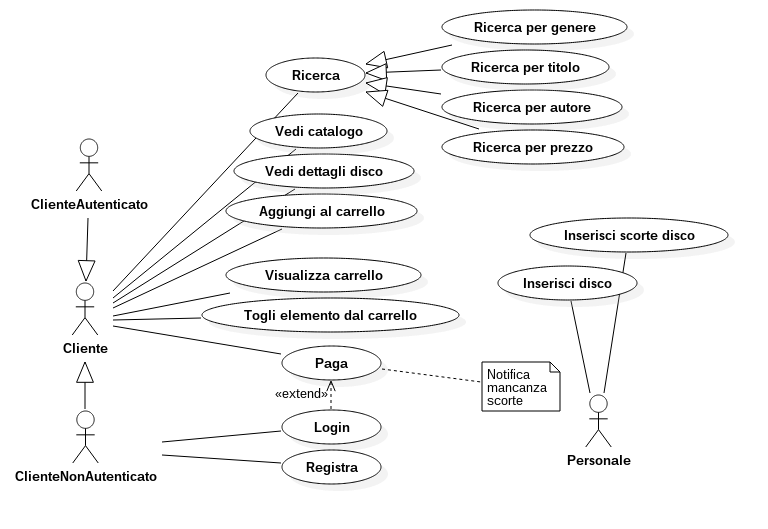
\includegraphics[width=\textwidth]{diagram/use-case.png}
\end{center}

\section{Requisiti in dettaglio}

\Requisito{Vedi Catalogo}{UC1}
    {Cliente}
    {Il software non è stato ancora avviato}
    {   \item Il cliente avvia il programma;
        \item Il sistema visualizza il catalogo.
    }
    {E' visualizzato il \gls{catalogo}}[Il catalogo degli utenti registrati è personalizzato in base al genere preferito]

\begin{center}
    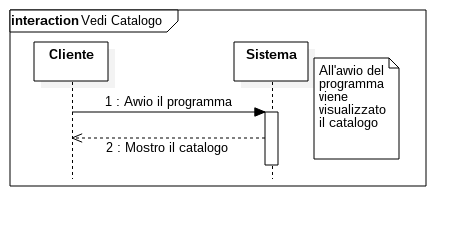
\includegraphics[width=0.5\textwidth]{diagram/seq-uc1.png}
\end{center}
    
\Requisito{Vedi dettagli disco}{UC2}
    {Cliente}
    {E' aperto il catalogo o una pagina di ricerca}
    {   \item Il cliente clicca sulla copertina di un album;
        \item Il sistema apre la pagina di dettagli dell'album.
    }
    {E' visualizzata la pagina di dettagli di un \gls{prodotto}}
    
\Requisito{Aggiungi al carrello}{UC3}
    {Cliente}
    {E' aperta la pagina di dettaglio di un prodotto}
    {   \item Il cliente clicca sul pulsante d'acquisto del prodotto.
        \begin{enumerate}[label*=\arabic*.]
            \item Se ci sono scorte del prodotto il sistema avvisa l'\gls{utente} del successo dell'operazione;
            \item Altrimenti visualizza un messaggio d'errore.
        \end{enumerate}
    }
    {E' visualizzata la pagina di dettagli del prodotto}[
        Il cliente può scegliere, nel caso l'operazione sia avvenuta con successo, di visualizzare il carrello.
    ]
    
\begin{center}
    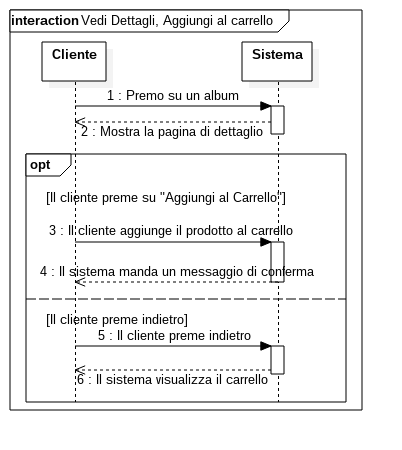
\includegraphics[width=0.5\textwidth]{diagram/seq-uc2-uc3.png}
\end{center}
    
\Requisito{Visualizza carrello}{UC4}
    {Cliente}
    {}
    {   \item Il cliente clicca il pulsante "Visualizza il carrello" dal menù o da uno dei messaggi del sistema.
        \item Il sistema visualizza il carrello.
    }
    {E' aperto il carrello}
    
\Requisito{Togli elemento dal carrello}{UC5} 
    {Cliente}
    {Il sistema visualizza il carrello}
    {   \item Il cliente avvisa il sistema di togliere un elemento dal carrello;
        \item Il sistema toglie l'elemento selezionato dal carrello.
    }
    {Il carrello ha un elemento in meno}

\Requisito{Paga}{UC6}
    {Cliente}
    {Il cliente vuole finalizzare l'acqusto}
    {   \item Il cliente preme sul pulsante "Acquista"
        \begin{enumerate}[label*=\arabic*.]
            \item Se il cliente non è autenticato, il sistema forza l'autenticazione o annulla l'operazione.
        \end{enumerate}
        \item Il cliente inserisce i dati relativi al pagamento;
        \item Il sistema verifica i dati inseriti;
        \begin{enumerate}[label*=\arabic*.]
            \item Se i dati sono corretti, il sistema avvisa il cliente dell'avvenuta operazione;
            \item Altrimenti il sistema visualizza un messaggio d'errore e annulla l'operazione.
        \end{enumerate}
        \begin{enumerate}[label*=\arabic*.]
            \item Se con l'acquisto corrente le scorte del disco scendono sotto una soglia critica, questo viene notificato al \gls{personale}.
        \end{enumerate}
    }
    {Il carrello è vuoto}[
    Ai clienti fedeli (almeno tre acquisti da almeno 250€ già fatti in passato) vengono proposti sconti e consegna gratuita]
    
\begin{center}
    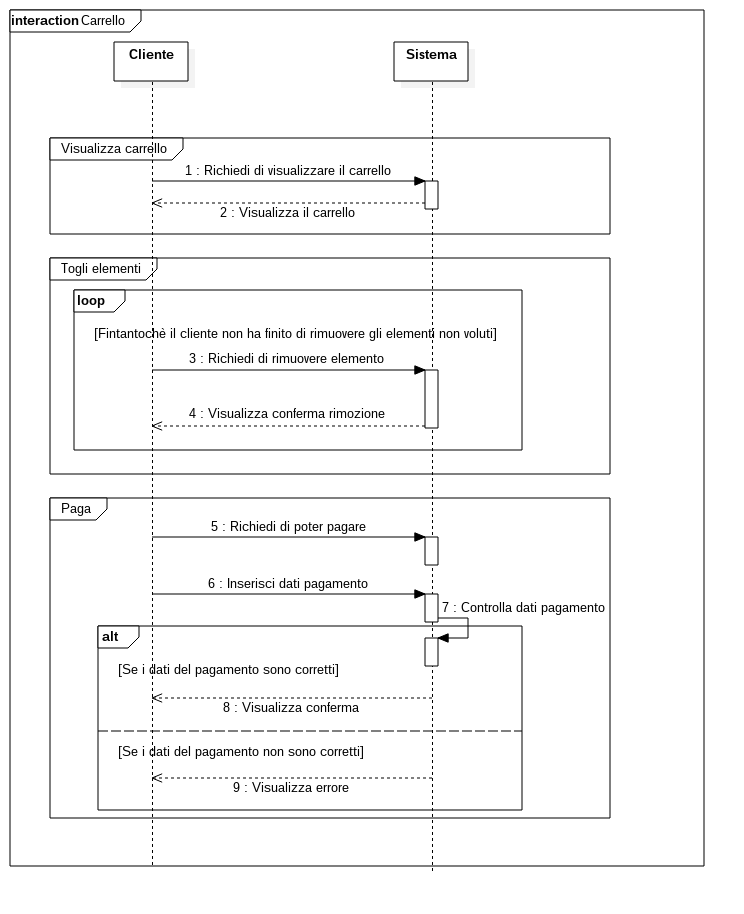
\includegraphics[width=0.7\textwidth]{diagram/seq-uc4-uc5-uc6.png}
\end{center}
    
\Requisito{Ricerca}{UC7}
    {Cliente}
    {}
    {   \item Il cliente avvia la ricerca;
        \item Il cliente seleziona il criterio con il quale effettuare la ricerca e inserisce i dati;
        \item Il sistema effettua la ricerca e restituisce la lista dei dischi che rispettano il criterio della ricerca.
    }
    {E' visualizzato l'elenco dei dischi cercati}
    
\Requisito{Login}{UC8}
    {ClienteNonAutenticato, Personale}
    {Il cliente vuole o il sistema richiede l'autenticazione per completare una operazione}
    {   \item Il cliente inserisce i suoi dati;
        \begin{enumerate}[label*=\arabic*.]
            \item Se i dati sono corretti, il sistema avvisa il cliente dell'avvenuta operazione;
            \item Altrimenti il sistema visualizza un \gls{messaggio} d'errore e annulla l'operazione.
        \end{enumerate}
    }
    {L'utilizzatore è autenticato}[
    Il personale visualizza un menù particolare che comprende voci per la gestione dei dischi]

\Requisito{Registra}{UC9}
    {ClienteNonAutenticato}
    {Il cliente vuole registrarsi}
    {   \item Il cliente apre il form per la registrazione;
        \item Il cliente inserisce i suoi dati;
        \begin{enumerate}[label*=\arabic*.]
            \item Se i dati sono corretti, il sistema avvisa il cliente dell'avvenuta operazione;
            \item Altrimenti il sistema visualizza un messaggio d'errore e annulla l'operazione.
        \end{enumerate}
    }
    {Il sistema ha un nuovo cliente registrato}

\Requisito{Inserisci disco}{UC10}
    {Personale}
    {L'utilizzatore del sistema si è autenticato come personale}
    {   \item Il personale apre il form per l'inserimento di un nuovo disco;
        \item Il personale inserisce i dati del disco;
        \begin{enumerate}[label*=\arabic*.]
            \item Se i dati sono corretti, il sistema avvisa il cliente dell'avvenuta operazione;
            \item Altrimenti il sistema visualizza un messaggio d'errore e annulla l'operazione.
        \end{enumerate}        
    }
    {Il sistema ha un nuovo disco}
    
\Requisito{Inserisci scorte}{UC11}
    {Personale}
    {}
    {   \item Il personale apre il form per l'inserimento delle scorte di un disco;
        \item Il personale inserisce i dati del disco;
        \begin{enumerate}[label*=\arabic*.]
            \item Se i dati sono corretti, il sistema avvisa il cliente dell'avvenuta operazione;
            \item Altrimenti il sistema visualizza un messaggio d'errore e annulla l'operazione.
        \end{enumerate}        
    }
    {Il sistema ha aumentato le scorte di un disco}
